\documentclass[landscape]{beamer}

\usepackage{drawstack}

\title{Compiling C with Clang by examples
\\[1em]
\(
 C \stackrel{\mbox{Clang}}{\longrightarrow} x86
 \)
 }
\author{Hayo Thielecke
\\
University of Birmingham
\\
\url{http://www.cs.bham.ac.uk/~hxt}
}


\begin{document}

\begin{frame}{}
\maketitle
\end{frame}

\begin{frame}{Contents}
\tableofcontents
\end{frame}

\section{Introduction}

\begin{frame}{Structure of the module}

\begin{block}{Parsing \checkmark}
\begin{itemize}
\item Progression from: Language + Logic, Models of Computation
\item abstract machines, formal,``mathy''
\end{itemize}
\end{block}

\begin{block}{Compiling C with Clang}
\begin{itemize}
\item Progression from: Computer Systems + Architecture, C/C++
\item not so formal, by example, x86 machine code
\end{itemize}
\end{block}

\begin{block}{Implementing functional languages}
\begin{itemize}
\item Progression from: functional programming
\item builds on abstract machines and C stack
\end{itemize}
\end{block}

\end{frame}
\begin{frame}[fragile]{Example}

\begin{minipage}{.5\textwidth}
C code
\begin{verbatim}
long f(long x, long y)
{
  long a, b;
  a = x + 42;
  b = y + 23;
  return a * b;
}
\end{verbatim}
\end{minipage}
%
\begin{minipage}{.4\textwidth}
x86 generated by Clang
\begin{verbatim}
f:                                      
	addq	$42, %rdi
	leaq	23(%rsi), %rax
	imulq	%rdi, %rax
	ret
\end{verbatim}
\end{minipage}
\vspace{2em}

The assembly code does not look much like the source code.
 
%How did the compiler know what to generate?

What happened to variables?

What happened to types?
\end{frame}

\begin{frame}{These are open source lectures and notes}

The \LaTeX{} source is in

\url{https://github.com/hayo-thielecke/clang-lectures}

\texttt{c-clang.tex} is for my slides

\texttt{c-clang-notes.tex} is for collaborative note taking.

\end{frame}

\begin{frame}{Aims and overview}

\begin{itemize}
\item
We will see some typical C code compiled to x86 assembly by LLVM/Clang
\item Emphasise general principles used in almost all compilers
\item Use Clang on C and x86 for example and concreteness
\item
\alert{What} Clang does, not details of \alert{how} it does it internally
\item
Enough to compile some C code by hand line by line
\item
C language features $\mapsto$ sequence of assembly instructions + addresses
\item
Various language features on top of vanilla functions
\item
Optimizations

\end{itemize}

\end{frame}

\section{Clang, LLVM, and x86 subset}

\begin{frame}{Clang and LLVM, the bestest and mostest compiler}

Clang is the bestest C/C++ compiler

\url{http://clang.llvm.org}

LLVM  is the mostest compiler infrastructure

\url{http://llvm.org}

Apple uses it

\url{https://developer.apple.com/xcode/}

Many projects, for example:

Emscripten: An LLVM to JavaScript Compiler

Rust: ``a safe, concurrent, practical language'' (as per blurb)

A not too technical intro to LLVM:
\url{http://www.aosabook.org/en/llvm.html}

\end{frame}

\begin{frame}{Using Clang}

Please do experiments yourself for seeing how LLVM/Clang compiles C.

Clang comes with XCode on OS X.

If you do not have LLVM on your computer:

ssh into a lab machine and type 

module load llvm/3.3

To compile, type

clang -S test.c

Then the assembly code will be in test.s

Function frodo will be labelled frodo: in test.s

For optimization, use

clang -S -O3 test.c

\end{frame}


%\section{Target architecture}

\begin{frame}{Target architecture for Clang output}

We will only need a tiny subset of assembly.

Quite readable.

Instruction we will need:

\[
\texttt{mov push pop call ret jmp add mul test be lea}
\]

The call instruction pushes the current instruction pointer onto the stack as the return address

ret pops the return address from the stack and makes it the new instruction pointer

A nice target architecture should have lots of general-purpose registers with indexed addressing.

Like RISC, but x86 is getting there in the 64-bit architecture

\end{frame}

\begin{frame}{Assembly generated by clang is x86 in AT\&T syntax}

mov syntax is target-last:

\texttt{mov} x y is like y = x ;

r prefix on registers means 64 bit register

movq etc: q suffix means quadword = 64 bits

\texttt{\%} register

\texttt{\$} constant

\texttt{\%rbp} = base pointer = frame pointer in general terminology

\texttt{\%rsp} = stack pointer, push and pop use it

indexed addressing \texttt{-24(\%rbp)}

\end{frame}


\begin{frame}[fragile]{Typical C code to compile}
\begin{minipage}{.5\textwidth}
\begin{verbatim}
long f(long x, long y)
{
  long a, b;
  a = x + 42;
  b = y + 23;
  return a * b;
}
\end{verbatim}
\end{minipage}
%
\begin{minipage}{.4\textwidth}
Parameters/arguments:
\\
 x and y

Local/automatic variables
\\
 a and b 
\end{minipage}
\\[4em]

More precisely, x and y are \emph{formal} parameters.

In a call f(1,2), 1 and 2 are the \emph{actual} parameters.

We will use the words ``parameter'' and ``argument'' interchangeably.

\end{frame}

\begin{frame}{Two big ideas in compiling functions}

\begin{block}{stack $\leftrightarrow$ recursion}

compare: parsing stack

many abstract and not so abstract machines use stacks

including JVM

In C: one stack frame per function call
\end{block}

\begin{block}{Names $\to$ indices}
Names can be compiled into indices, discovered many times

%deBruijn indices: lambda calculus without variables
%
%cartesian closed categories, CAM machine for CAML

In C: variables become small integers to be added to the base pointer

\end{block}

\end{frame}

\section{Call stack and stack frames}

\begin{frame}[fragile]{Stack frame details}

The details differ between architectures (e.g., x86, ARM, SPARC)

Ingredients of stack frames, in various order, some may be missing:

return address 

parameters

local vars

saved frame pointer

caller or callee saved registers

static link (in Pascal and Algol, but not in C)

this pointer for member functions (in C++)
\end{frame}


\begin{frame}[fragile]{A traditional stack layout (but not Clang)}

%On most hardware, the stack grows towards smaller addresses.

Convention: we draw the stack growing \alert{downwards} on the page. 

Suppose function \texttt g calls function \texttt f.


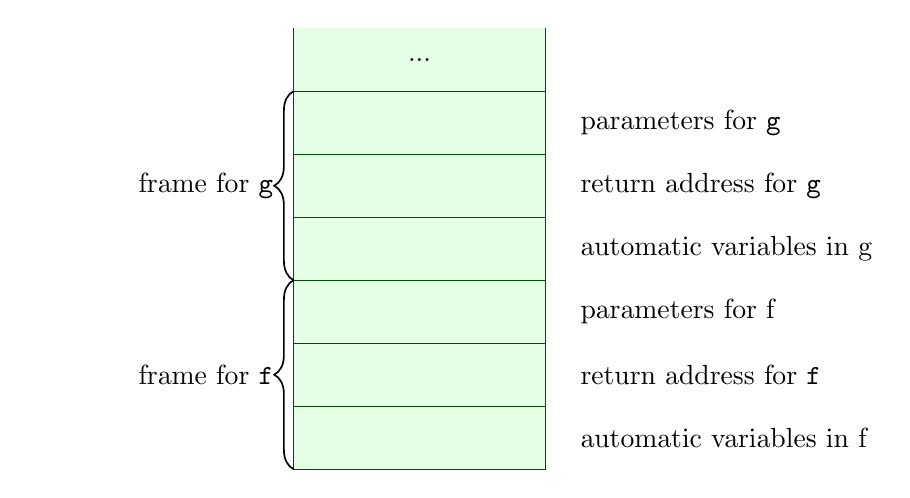
\begin{tikzpicture}[scale=.8]
  \stacktop{}
  \startframe
      \cell{}  
\cellcom{parameters for \texttt g} 
    \cell{}  
\cellcom{return address for \texttt g} 
      \cell{}        
    \cellcom{automatic variables in g}         
\finishframe{frame for \texttt g\ } 
  \startframe
  \cell{}  
    \cellcom{parameters for f} 
  \cell{}  
\cellcom{return address  for \texttt f} 
  \cell{}  
    \cellcom{automatic variables in f}
 \finishframe{frame for \texttt f\ } 
\end{tikzpicture}
There may be more in the frame, e.g. saved registers  
\end{frame}   


\begin{frame}[fragile]{What about recursive functions?}

Consider the standard example of recursion:

\begin{verbatim}
long factorial(long n)
{
  if(n == 0)
    return 1;
  else
    return factorial(n - 1) * n;
}
\end{verbatim}


\end{frame}

\begin{frame}[fragile]{Call stack: one frame per function \alert{call}}

Recursion example: fac(n) calls fac(n - 1). Each recursive call gets a smaller parameter.

The return address points into the code segments, \alert{not the stack} or heap.

What are the return addresses?
\\[1em]

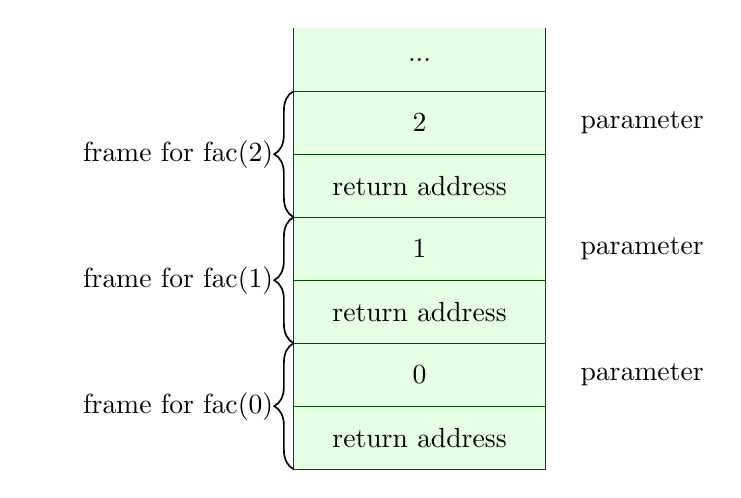
\begin{tikzpicture}[scale=.8]
  \stacktop{}
    \startframe
      \cell{2}  
    \cellcom{parameter}
  \cell{return address}  
  \finishframe{frame for {fac(2)}} 
  \startframe
      \cell{1}  
    \cellcom{parameter}
  \cell{return address}  
  \finishframe{frame for {fac(1)}} 
  \startframe
  \cell{0}  
    \cellcom{parameter} 
  \cell{return address}  
 \finishframe{frame for fac(0)} 
\end{tikzpicture}

\end{frame}   

\begin{frame}[fragile]{Return address example}

\begin{verbatim}
long factorial(long n)
{
  if(n == 0)
    return 1;
  else
    return factorial(n - 1) * n;
}
\end{verbatim}

The return address is a pointer to the compiled code. The returned value is returned into the hole $\bigcirc$ position in the last statement,
\[
\texttt{return $\bigcirc$ * n;}
\]
Thus when the function returns, 1 is plugged into the hole, then 2, then 6, \ldots

The return address represents a continuation.
\end{frame}

\begin{frame}{Calling conventions and stack frame layout}

The calling convention differs between compilers and architectures

Old school: 
\\push arguments onto stack, then do a call instruction (which pushes return address)

Modern architectures have many registers
\\
$\Rightarrow$ pass arguments in registers when possible; Clang does this

Some RISC architectures put return address into a link register

more exotic: SPARC has register windows for parameter passing
\end{frame}


\begin{frame}[fragile]{Stack frame in clang C calling convention on x86}

Clang \alert{passes parameters in registers} \texttt{rdi}, \texttt{rds}, \ldots

The parameters \alert{also have a slot in the frame}

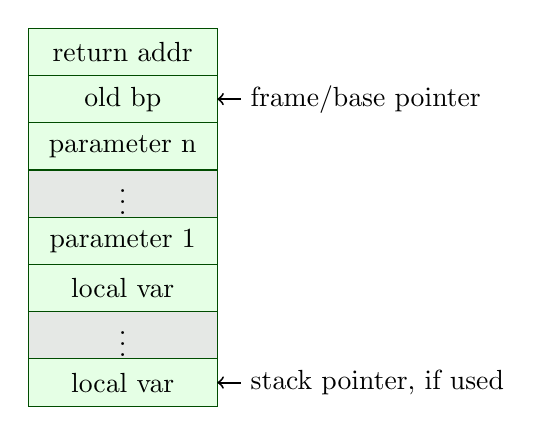
\begin{tikzpicture}[scale=.6]
  \startframe
     \cell{return addr} 
    \cell{old bp}  \cellptr{\textrm{frame/base pointer}} 
      \cell{parameter n}
     \cell[padding]{\vdots}
         \cell{parameter 1} %\cellptr{\texttt{stack} + 2}
    \cell{local var}
     \cell[padding]{\vdots}
    \cell{local var}\cellptr{\textrm{stack pointer, if used}} 
%\finishframe{array} 
\end{tikzpicture}
  
\end{frame} 


\begin{frame}[fragile]{Clang function idiom}

\url{http://llvm.org/docs/LangRef.html#calling-conventions}

\begin{verbatim}
f:
	pushq	%rbp
	movq	%rsp, %rbp
    ... body of function f
	popq	%rbp
	ret
\end{verbatim}

parameters are passed in registers rdi, rsi

return value is passed in register rax
\end{frame}



\begin{frame}[fragile]{Computing the index in the frame}

Simple in principle: 
\\
walk over the syntax tree and keep track of declarations

The declarations tell us the size: long x means x needs 8 bytes

That is why C has type declarations in the first place

\begin{verbatim}
long f(long x, long y) // put y at -8 and x at -16
{
    long a;    // put a at -24
    long b;    // put b at -32
    a = x;    // now we know where a and x are 
              // relative to rbp
}    
\end{verbatim}

Exercise: what happens if we also have char and float declarations?    
\end{frame}

\begin{frame}[fragile]{Clang stack frame example}
\begin{verbatim}
long f(long x, long y) // put y at -8 and x at -16
{
    long a;    // put a at -24
    long b;    // put b at -32
    ...
}
\end{verbatim}
  
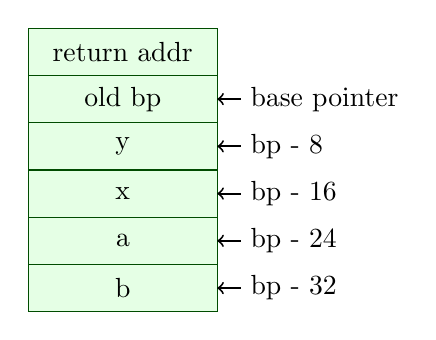
\begin{tikzpicture}[scale=.6]
 % \startframe
     \cell{return addr} 
    \cell{old bp}  \cellptr{\textrm{base pointer}} 
      \cell{y}\cellptr{\textrm{bp - 8}}
         \cell{x} \cellptr{\textrm{bp - 16}}
    \cell{a}  \cellptr{\textrm{bp - 24}}
    \cell{b} \cellptr{\textrm{bp - 32}}
% \finishframe{array} 
\end{tikzpicture}
  
\end{frame} 


\begin{frame}[fragile]{Compiled with clang -S}
\begin{minipage}{.55\textwidth}
\begin{verbatim}
long f(long x, long y)
{
  long a, b;
  a = x + 42;
  b = y + 23;
  return a * b;
}
\end{verbatim}

\begin{eqnarray*}
\texttt x&\mapsto& \texttt{rdi}
\\
\texttt y&\mapsto& \texttt{rsi}
\\
\texttt x&\mapsto& \texttt{rbp}-8
\\
\texttt y&\mapsto& \texttt{rbp}-16 
\\
\texttt a&\mapsto& \texttt{rbp}-24
\\
\texttt b&\mapsto& \texttt{rbp}-32
\end{eqnarray*}

\end{minipage}
%
\begin{minipage}{.4\textwidth}
\begin{verbatim}
f:
	pushq	%rbp
	movq	%rsp, %rbp
	movq	%rdi, -8(%rbp)
	movq	%rsi, -16(%rbp)
	movq	-8(%rbp), %rsi
	addq	$42, %rsi
	movq	%rsi, -24(%rbp)
	movq	-16(%rbp), %rsi
	addq	$23, %rsi
	movq	%rsi, -32(%rbp)
	movq	-24(%rbp), %rsi
	imulq	-32(%rbp), %rsi
	movq	%rsi, %rax
	popq	%rbp
	ret
\end{verbatim}
\end{minipage}
\end{frame}



\begin{frame}[fragile]{Optimization: compiled with clang -S -O3}
\begin{minipage}{.5\textwidth}
\begin{verbatim}
long f(long x, long y)
{
  long a, b;
  a = x + 42;
  b = y + 23;
  return a * b;
}
\end{verbatim}
\end{minipage}
%
\begin{minipage}{.4\textwidth}
\begin{verbatim}
f:                                      
	addq	$42, %rdi
	leaq	23(%rsi), %rax
	imulq	%rdi, %rax
	ret
\end{verbatim}
\end{minipage}
\end{frame}

\begin{frame}{Leaf functions}

A ``leaf'' function is one that does not call any functions.

It is a leaf in the control flow graph/tree: 
\\
leaf = node without children.

Leaf functions can be compiled more simply:
\\
no need to adjust stack pointer
\\
no need to save registers into frame
\\
Some leaf functions can work entirely on registers, which is efficient.
\end{frame}

\begin{frame}[fragile]{Many arguments $\Rightarrow$ spill into the stack}
Some passed on the stack, not in registers. These have positive indices. Why?
\\[2em]

\begin{minipage}{.55\textwidth}
\begin{verbatim}
long a(long x1, long x2, 
long x3, long x4, long x5, 
long x6, long x7, long x8)
{
  return x1 + x7 + x8;
}
\end{verbatim}
\end{minipage}
%
\begin{minipage}{.4\textwidth}
\begin{verbatim}
a:                             
	addq	8(%rsp), %rdi
	addq	16(%rsp), %rdi
	movq	%rdi, %rax
	ret
\end{verbatim}
\end{minipage}
\vspace{2em}

We will not use lots of arguments. While a C compiler must allow it, it is not good style.

\end{frame}


\begin{frame}[fragile]{Stretch exercise on calling conventions}

Here is a function definition very similar to one in the original manual on B, the predecessor of C.
\begin{verbatim}
void printn(n, x0, x1, x2, x3, x4, x5, x6, x7, x8, x9)
/* print n arguments as integers */
{
  int i, *p;
  p = &x0;
  for(i=0; i<n; i++) printf("%d\n", p[i]); 
}
\end{verbatim}
Explain how this function could work. You may assume that all parameters are passed on the stack, and in reverse order. 

Will it still work in Clang?
\end{frame}

\begin{frame}[fragile]{Calling functions}
A function call
\begin{verbatim}
f(E1, ... , En)
\end{verbatim}
is broken down into into steps like this
\begin{verbatim}
arg1 = E1;
...
argn = En;
call f;
\end{verbatim}
where \texttt{argi} are the argument positions of the calling convention.

Note: in C, the order for computing \texttt{argi} is unspecified to give the compiler the freedom to optimize.

If a function calls some function (i.e., it is non-leaf), it needs to adjust the stack pointer.
\end{frame}

\begin{frame}[fragile]{Calling another function example}
\begin{minipage}{.5\textwidth}
\begin{verbatim}
long f(long x)
{
  return g(x + 2) - 7;
}
\end{verbatim}
\end{minipage}
%
\begin{minipage}{.4\textwidth}
\begin{verbatim}
f:  
	pushq	%rbp
	movq	%rsp, %rbp
	subq	$16, %rsp
	movq	%rdi, -8(%rbp)
	movq	-8(%rbp), %rdi
	addq	$2, %rdi
	callq	g
	subq	$7, %rax
	addq	$16, %rsp
	popq	%rbp
	ret
\end{verbatim}
\end{minipage}
\vspace{1em}

%Why is there the following code?
%\begin{verbatim}
%	subq	$16, %rsp
%	...
%	addq	$16, %rsp	
%\end{verbatim}


\end{frame}


\section{Pointers as parameters and call by reference}


\begin{frame}[fragile]{Call by reference in C = call by value + pointer}
\small
\begin{verbatim}
void f(int *p)
{
    *p = *p + 2; // draw stack after this statement
}

void g()
{
    int x = 10;
    f(&x);
}
\end{verbatim}

\begin{drawstack}[scale=.6]
\stacktop{}
  
% \startframe
    \cell{12}  \cellcomL{x}
    \coordinate (a) at (currentcell.east);
          \cell{\dots}  
     \separator 
       \cell{\dots} 
%\finishframe{g} 
%\startframe
     \cell{$\bullet$}  \cellcomL{p}
 \coordinate (p) at (currentcell.center);
%\finishframe{f} 
  \draw[->] (p) .. controls (4,-4) and (4,-1)  .. (a);
\end{drawstack}
  
\end{frame} 



\begin{frame}[fragile]{For comparison: call by value modifies only local copy}
\small
\begin{verbatim}
void f(int y)
{
    y = y + 2; // draw stack after this statement
}

void g()
{
    int x = 10;
    f(x);
}
\end{verbatim}

\begin{drawstack}[scale=.6]
\stacktop{}
  
% \startframe
    \cell{10}  \cellcomL{x}
    \coordinate (a) at (currentcell.east);
          \cell{\dots}  
     \separator 
       \cell{\dots} 
%\finishframe{g} 
%\startframe
     \cell{$12$}  \cellcomL{y}
 \coordinate (p) at (currentcell.center);
%\finishframe{f} 
%  \draw[->] (p) .. controls (4,-4.5) and (4,-1)  .. (a);
\end{drawstack}
  
\end{frame} 

\begin{frame}{Escaping variables and stack frames}

The compiler normally tries to place variables in registers when optimizing.

The frame slot may be ignored.

However, if we apply \texttt{\&} to a variable, its value must be kept in the frame slot.

The variable ``escapes'' from the frame in the sense that it can be referred to from outside.

\begin{drawstack}[scale=.5]
\stacktop{}
  
% \startframe
    \cell{12}  \cellcomL{x}
    \coordinate (a) at (currentcell.east);
          \cell{\dots}  
     \separator 
%\finishframe{g} 
%\startframe
     \cell{$\bullet$}  \cellcomL{p}
 \coordinate (p) at (currentcell.center);
%\finishframe{f} 
  \draw[->] (p) .. controls (4,-4) and (4,-1)  .. (a);
\end{drawstack}
\end{frame}

\begin{frame}[fragile]{Call with pointer: calling function}
\begin{minipage}{.5\textwidth}
\begin{verbatim}
void f(long x, long *p)
{
  *p = x;
}

long g()
{
  long a = 42;
  f(a + 1, &a);
  return a;
}
\end{verbatim}
\end{minipage}
%
\begin{minipage}{.4\textwidth}
\begin{verbatim}
g:                                
	pushq	%rbp
	movq	%rsp, %rbp
	subq	$16, %rsp
	leaq	-8(%rbp), %rsi
	movq	$42, -8(%rbp)
	movq	-8(%rbp), %rax
	addq	$1, %rax
	movq	%rax, %rdi
	callq	f
	movq	-8(%rbp), %rax
	addq	$16, %rsp
	popq	%rbp
	ret
\end{verbatim}
\end{minipage}
\end{frame}



\begin{frame}[fragile]{Call with pointer: called function}
\begin{minipage}{.5\textwidth}
\begin{verbatim}
void f(long x, long *p)
{
  *p = x;
}

long g()
{
  long a = 42;
  f(a + 1, &a);
  return a;
}
\end{verbatim}
\end{minipage}
%
\begin{minipage}{.4\textwidth}
\begin{verbatim}
f:  
	pushq	%rbp
	movq	%rsp, %rbp
	movq	%rdi, -8(%rbp)
	movq	%rsi, -16(%rbp)
	movq	-8(%rbp), %rsi
	movq	-16(%rbp), %rdi
	movq	%rsi, (%rdi)
	popq	%rbp
	ret
\end{verbatim}
\end{minipage}
\end{frame}

\begin{frame}[fragile]{Call with pointer: optimized with -O3}
\begin{minipage}{.5\textwidth}
\begin{verbatim}
void f(long x, long *p)
{
  *p = x;
}

\end{verbatim}
\end{minipage}
%
\begin{minipage}{.4\textwidth}
\begin{verbatim}
f:  
	movq	%rdi, (%rsi)
	ret
\end{verbatim}
\end{minipage}
\end{frame}

\begin{frame}[fragile]{Pointers exercise: my god, it's full of stars}
Suppose there are multiple pointer dereferences:

\begin{verbatim}
void f(long x, long ***p)
{
  ***p = x;
}

\end{verbatim}

How should this be compiled? Hint: multiple indirect addressing, \texttt{(\%rdi)}.
\\
Draw the memory with arrows for pointers as illustration.
\end{frame}

\section{Function pointers}


\begin{frame}[fragile]{Function pointer as function parameter}
\begin{verbatim}
void g(void (*h)(int))
{
    int x = 10;
    h(x + 2);
}
    
void f(int y) { ... }

... g(f) ...
\end{verbatim}

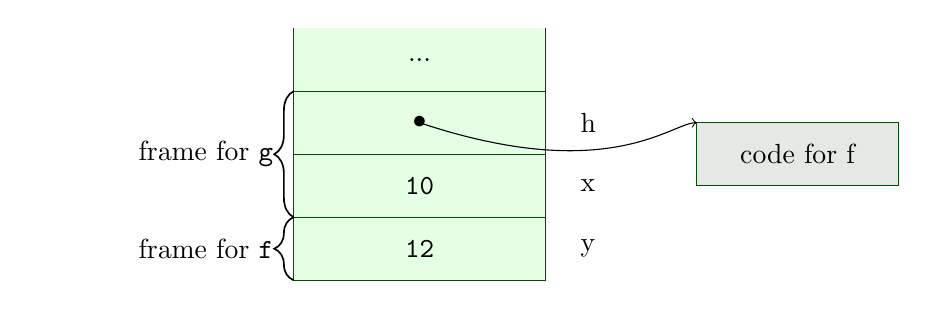
\begin{tikzpicture}[scale=.8]
  \stacktop{}
  \startframe
%\cellcom{return address for \texttt g} 
      \cell{$\bullet$} 
          \coordinate (a) at (currentcell.center);       
    \cellcom{h}  
  \cell{\texttt{10}}        
    \cellcom{x}  
\finishframe{frame for \texttt g\ } 
  \startframe
   \cell{\texttt{12}}  
    \cellcom{y} 
 \finishframe{frame for \texttt f\ } 
   \drawstruct{(6,-.5)})
  \structcell[padding]{code for f}
 \coordinate (O1) at (structtopleft);
   \draw[->] (a) .. controls (3,-2) and (4,-1) ..  (O1);
\end{tikzpicture}
  
\end{frame}   


\begin{frame}[fragile]{Function pointer as a parameter}
\begin{minipage}{.5\textwidth}
\begin{verbatim}
long f(long (*g)(long))
{
  return g(42) + 2;
}
\end{verbatim}
\end{minipage}
%
\begin{minipage}{.4\textwidth}
\begin{verbatim}
f:                   
	pushq	%rbp
	movq	%rsp, %rbp
	movabsq	$42, %rax
	movq	%rdi, -8(%rbp)
	movq	%rax, %rdi
	callq	*-8(%rbp)
	addq	$16, %rsp
	popq	%rbp
	ret
\end{verbatim}
\end{minipage}
\vspace{3em}

Not optimized. We'll see tailcall optimization later.
\end{frame}


\begin{frame}[fragile]{Buffer overflow on the call stack}
\small
\begin{verbatim}
int vulnerable_function()
{
    int winner = 0; // suppose this is security-critical
    char name[8];   // this is the buffer to be overflown
    
    printf("Please enter your name:\n");
    fgets(name, 200, stdin);
    ...
}
\end{verbatim}
Input \texttt{blahblahbl} overflows the string variable on the stack:
\begin{center}
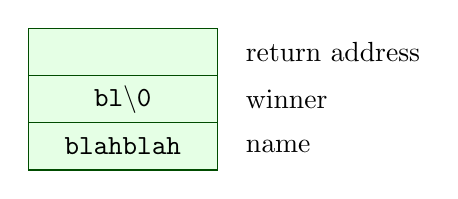
\begin{tikzpicture}[scale=.6]
\cell{}  \cellcom{return address}
\cell{\texttt{bl\textbackslash 0}}  \cellcom{winner}
\cell{\texttt{blahblah}}  \cellcom{name}
\end{tikzpicture}
  \end{center}
 Note: the call stack grows towards \alert{lower} machine addresses.
\end{frame} 

\begin{frame}[fragile]{Stretch exercise on buffer overflow}
Here is some code vulnerable to classic buffer overflow:
\begin{verbatim}
void bufwin()
{
  int winner = 0; // suppose this is security-critical
  char name[10]; // automatic, so stack-allocated  
  printf("Please enter your name:\n");
  fgets(name, 200, stdin); // overflow array name
  if (winner) // attacker overflowed name into winner
    printf("You WIN, %s\n", name);
  else
    printf("You LOSE, %s\n", name);
}
\end{verbatim}
On modern compilers, this attack will not succeed. Look into the assembly code and see how the defence works.
\end{frame}



\section{Optimizations: inlining and tail calls}


\begin{frame}{Function inlining}

\begin{itemize}
\item
Function inlining = do a function call at compile time.
\item
Saves the cost of a function call at runtime.
\item
Copy body of called function + fill in arguments.
%\item Compiler needs to be careful about side effects in the arguments.
\item C even has a keyword \texttt{inline}, but Clang is smart enough to know when to inline anyway
\item
Modern C compilers do inlining, so C macros can be avoided.
\item
Modern C++ uses template, which give the compiler many opportunities for inlining.
\item
Inlining has a clean theoretical foundation: beta reduction in the lambda calculus.

\end{itemize}


\end{frame}

\begin{frame}[fragile]{Function inlining example}
\begin{minipage}{.5\textwidth}
\begin{verbatim}
long sq(long x)
{
  return x * x;
}

long f(long y)
{
  long z = sq(++y);
  return z;
}
\end{verbatim}
\end{minipage}
%
\begin{minipage}{.4\textwidth}
\begin{verbatim}
f:                   
	incq	%rdi
	imulq	%rdi, %rdi
	movq	%rdi, %rax
	ret
\end{verbatim}
\end{minipage}
\\[2em]

Note: cannot just do \texttt{++y * ++y}
\end{frame}

\begin{frame}[fragile]{Inlining exercise}

Simplify the following C code as much as possible by performing function inling.

\begin{verbatim}
long sq(long x) { return x * x; }

long f(long (*g)(long))
{
  return g(42) + 2;
}

long applyftosq()
{
  return f(sq);
}
\end{verbatim}

\end{frame}


\begin{frame}[fragile]{Tail call optimization}

Tail position = the last thing that happens inside a function body before the return.


Here f is in tail position:
\begin{verbatim}
return f(E);
\end{verbatim}
f is not in tail position here:
\begin{verbatim}
return 5 + f(E);
\end{verbatim}
or here:
\begin{verbatim}
return f(E) - 6;
\end{verbatim}
A function call in tail position can be compiled as a jump.

\end{frame}



\begin{frame}[fragile]{Function as a parameter, non-tailcall }
\begin{minipage}{.5\textwidth}
\begin{verbatim}
long f(long (*g)(long))
{
  return g(42) - 6;
}
\end{verbatim}
\end{minipage}
%
\begin{minipage}{.4\textwidth}
\begin{verbatim}
f: 
	pushq	%rax
	movq	%rdi, %rax
	movl	$42, %edi
	callq	*%rax
	addq	$-6, %rax
	popq	%rdx
	ret
\end{verbatim}
\end{minipage}

\end{frame}


\begin{frame}[fragile]{Function as a parameter, tailcall optimized}
\begin{minipage}{.5\textwidth}
\begin{verbatim}
long f(long (*g)(long))
{
  return g(42);
}
\end{verbatim}
\end{minipage}
%
\begin{minipage}{.4\textwidth}
\begin{verbatim}
f:                              
	movq	%rdi, %rax
	movl	$42, %edi
	jmpq	*%rax  # TAILCALL
\end{verbatim}
\end{minipage}
\end{frame}


\begin{frame}{Stretch exercise: vectorizing optimizations}

Take some simple code, say factorial.

Compile it on the latest version of clang with all optimizations enabled.

Try to understand what the resulting code does.

It will probably look very different to the source code.

Loop unrolling to enable parallel computation.

\end{frame}

\section{Compiling structures and objects}

\begin{frame}[fragile]{Compiling structures and objects}

Same idea as in stack frames:

access in memory via
pointer + index

Structure \alert{definition} tells the compiler the size and indices of the members.

No code is produced for a struct definition on its own. 

But the compiler's symbol table is extended: it knows about the member names and their types.

Structure \alert{access} then uses indexed addressing using those indices.

\begin{verbatim}
struct S {
  T1 x;
  T2 y;
};
\end{verbatim}
\pause
\texttt x is a index 0\\
 \texttt y is at \texttt{sizeof(T2)} + padding for alignment
\end{frame}

\begin{frame}[fragile]{Structure access}
\begin{minipage}{.5\textwidth}
\begin{verbatim}
struct S {
  long x;
  long y;
};

void s(struct S *p)
{
  p->x = 23;
  p->y = 45;
}
\end{verbatim}
\end{minipage}
%
\begin{minipage}{.45\textwidth}
\begin{verbatim}
s:      
   pushq   %rbp
   movq    %rsp, %rbp
   movq    $23, (%rdi)
   movq    $45, 8(%rdi)
   popq    %rbp
   retq
\end{verbatim}
\end{minipage}
\begin{eqnarray*}
\texttt x&\mapsto& 0
\\
\texttt y&\mapsto& 8
\end{eqnarray*}
\end{frame}


\begin{frame}{Member functions of objects}

\begin{itemize}
\item
In C++, functions defined inside classes (``member functions'') have access to other members of the class.
\item
Implemented using \texttt{this} pointer.
\item
The \texttt{this} pointer points at the object (not the class).
\item
In a call of a member function, the \texttt{this} pointer is passed like an additional parameter.
\item
Dereferencing this extra parameter accesses gives access to members.
\end{itemize}

\end{frame}

\begin{frame}[fragile]{Member function access to object example}
\begin{minipage}{.5\textwidth}
\begin{verbatim}
class C {
  long n;
public:
  long f() 
  { 
    return n; 
  }
};
\end{verbatim}
\end{minipage}
%
\begin{minipage}{.4\textwidth}
Code for f:
\begin{verbatim}
	pushq	%rbp
	movq	%rsp, %rbp
	movq	%rdi, -8(%rbp)
	movq	-8(%rbp), %rdi
	movq	(%rdi), %rax
	popq	%rbp
	ret
\end{verbatim}
\end{minipage}

\vspace{3em}

Exercise: draw the stack and heap to illustrate how the function above works.
\end{frame}


\begin{frame}[fragile]{Exercise on structures}
Suppose the following structure definition is given:
\begin{verbatim}
struct S {
  struct S *next;
  struct S *prev;
  long data;
};
\end{verbatim}
%
Suppose a pointer \texttt p is held in register \texttt{\%rsi}. Translate the following C statements to assembly:
\begin{verbatim}
p->data = 12345;
p->next = p->prev->next;
\end{verbatim}
\end{frame}

\begin{frame}[fragile]{Stretch exercise on structures}

Building on what you have learned about structures, how are C unions compiled?

For example, consider 
\begin{verbatim}
union u {
  A x;
  B y;
};
\end{verbatim}

What are the adresses for \texttt{A} and \texttt{B}?
\end{frame}

\begin{frame}{More on C++}

If you are interested in object-orientation, you can do more experiments by observing how Clang compiles C++ code.

Example: virtual function table, implemented using yet more pointers.

But compiled C++ is harder to read than for C, due to name mangling. 
\end{frame}




\end{document}

